\section{Storing the Data}\label{sec: 5-storing}
In this section, we discuss how the filtered documents are stored and how Neo4j was used for storing extracted relations, following the design described in section \ref{sec:storage-design}. We discuss the storage and graph database parts from the overview (see figure \ref{fig:overview}).

\subsection{Storing Filtered Documents}
The documents that pass the filtering stage can be stored for several reasons. For example, the classifier can be retrained and might thus label documents differently. To avoid having to download and process all the pages again, it is useful to store the documents on disk. If the disk is small, it is wise to compress the documents. However, compression is a slow process, so if enough disk space is available, storing the documents uncompressed is more feasible.

In the \texttt{TextDownloader} class, that was already shortly discussed in section \ref{sec:5-downloading}, storage to disk is done without compression in all cases. We did this since this project only involves a relatively small data set, e.g. one that can be stored without the need for compression.

\subsection{Storing Extracted Data}
To be able to interact with the results of the application, it is required to store extracted relations. The implementation of the storage follows the design of section section \ref{sec:storing-data}, using the graph database Neo4j.

\subsubsection{Neo4j Model}
The model used for the graph structure follows the concepts described in section \ref{sec:neo4j-concepts}. It consists of nodes, labels and properties. To distinguish between and to efficiently query for specific (types of) nodes, at least one label is assigned to the node. Below, the labels we used are listed and per label, a description of the nodes they are attached to is given:

\begin{description}
\item[:City] Nodes labelled as \texttt{:City} represent the cities the application uses. These nodes contain multiple properties: name, population, longitude and latitude. Population is used in the visualisation (see section \ref{sec 5-front-end}) for scaling. Longitude and latitude are used to place the cities on a map and were retrieved through the Google Maps Geocoding API\footnote{\url{https://developers.google.com/maps/documentation/geocoding/start?hl=en_US}}.
\item[:Index] Nodes with the \texttt{:Index} label represent documents that are found useful. Every document has this label, in addition to the label representing the category they are classified as. The following basic properties belong to these nodes: file name, offset and length. They point to the exact file location where the page can be downloaded from CommonCrawl. Additionally, the nodes contain a probability property per category. These probabilities come from the classifier and are there for validation purposes.
\item[Categories] For each category, a label exists to separate a category from the bulk of documents. This way, documents of a specific category can be matched against. This is particularly useful to count, for example, the documents about "Leisure" (and thus labelled \texttt{:Leisure}), that two cities have in common. Since category labels are only applied to nodes that also have the \texttt{:Index} label, they contain no additional properties.
\end{description}

The nodes are connected using relations. Cities (\texttt{:City} labelled nodes) occurring in documents (\texttt{:Index} labelled nodes) are connected with a \texttt{:OCCURS\_IN} relation. It is mainly used to find documents in which a pair of cities occurs. For example, the query below matches the documents Rotterdam and Amsterdam have in common and returns the file names:

\begin{lstlisting}[language=cypher, caption={Querying documents containing two cities}, label={lst:query-occ}]
MATCH (:City { name: 'Amsterdam })-[:OCCURS_IN]->
    (i:Index)
        <-[:OCCURS_IN]-(b:City { name: 'Rotterdam'})
RETURN i.filename
\end{lstlisting}

\begin{figure}
    \centering
    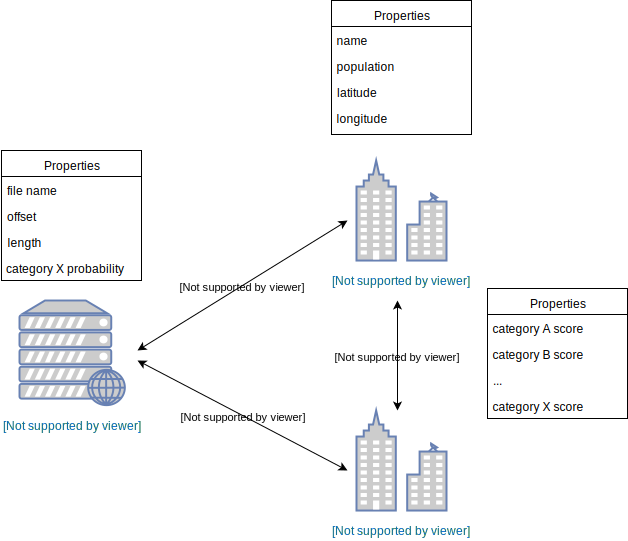
\includegraphics[width=0.6\textwidth]{neo4j-model-full}
    \caption{The Neo4j model as implemented}
    \label{fig:my_label}
\end{figure}

% relation types
% properties
% db_utils

% steden op basis van lijst van klant, coordinaten opgezocht via google api
% issue: steden met dubbele naam kregen zelfde coordinaten en niet per se de grootste, maar belangrijkste (volgens google)
% neo4j city node
% neo4j index node
% occurrence relation
% intercity relation
% parameterised optimisation -> benchmark
% bulk vs single -> single transaction instead of transaction for every statement, benchmark
% transactional vs multithreaded -> data inconsistencies
% neo4j python driver issues
% solution: use neo4j's own multi-threading using UNWIND -> embedded multithreading
% remarks: 
% try SQL instead of NoSQL to compare results
% perhaps java instead of python driver to be able to use multithreading
\todo{mention multithreading neo4j (embedded)}